\documentclass[tikz,border=5pt]{standalone}
\usepackage{amsmath,amssymb}
\usetikzlibrary{decorations.pathreplacing,calc,arrows.meta,positioning}

\definecolor{accent}{RGB}{0, 100, 170}
\definecolor{highlight}{RGB}{200, 60, 30}
\definecolor{darkgreen}{RGB}{0, 120, 60}
\definecolor{earthblue}{RGB}{40,80,150}
\definecolor{orbitgray}{RGB}{100,100,100}

\begin{document}
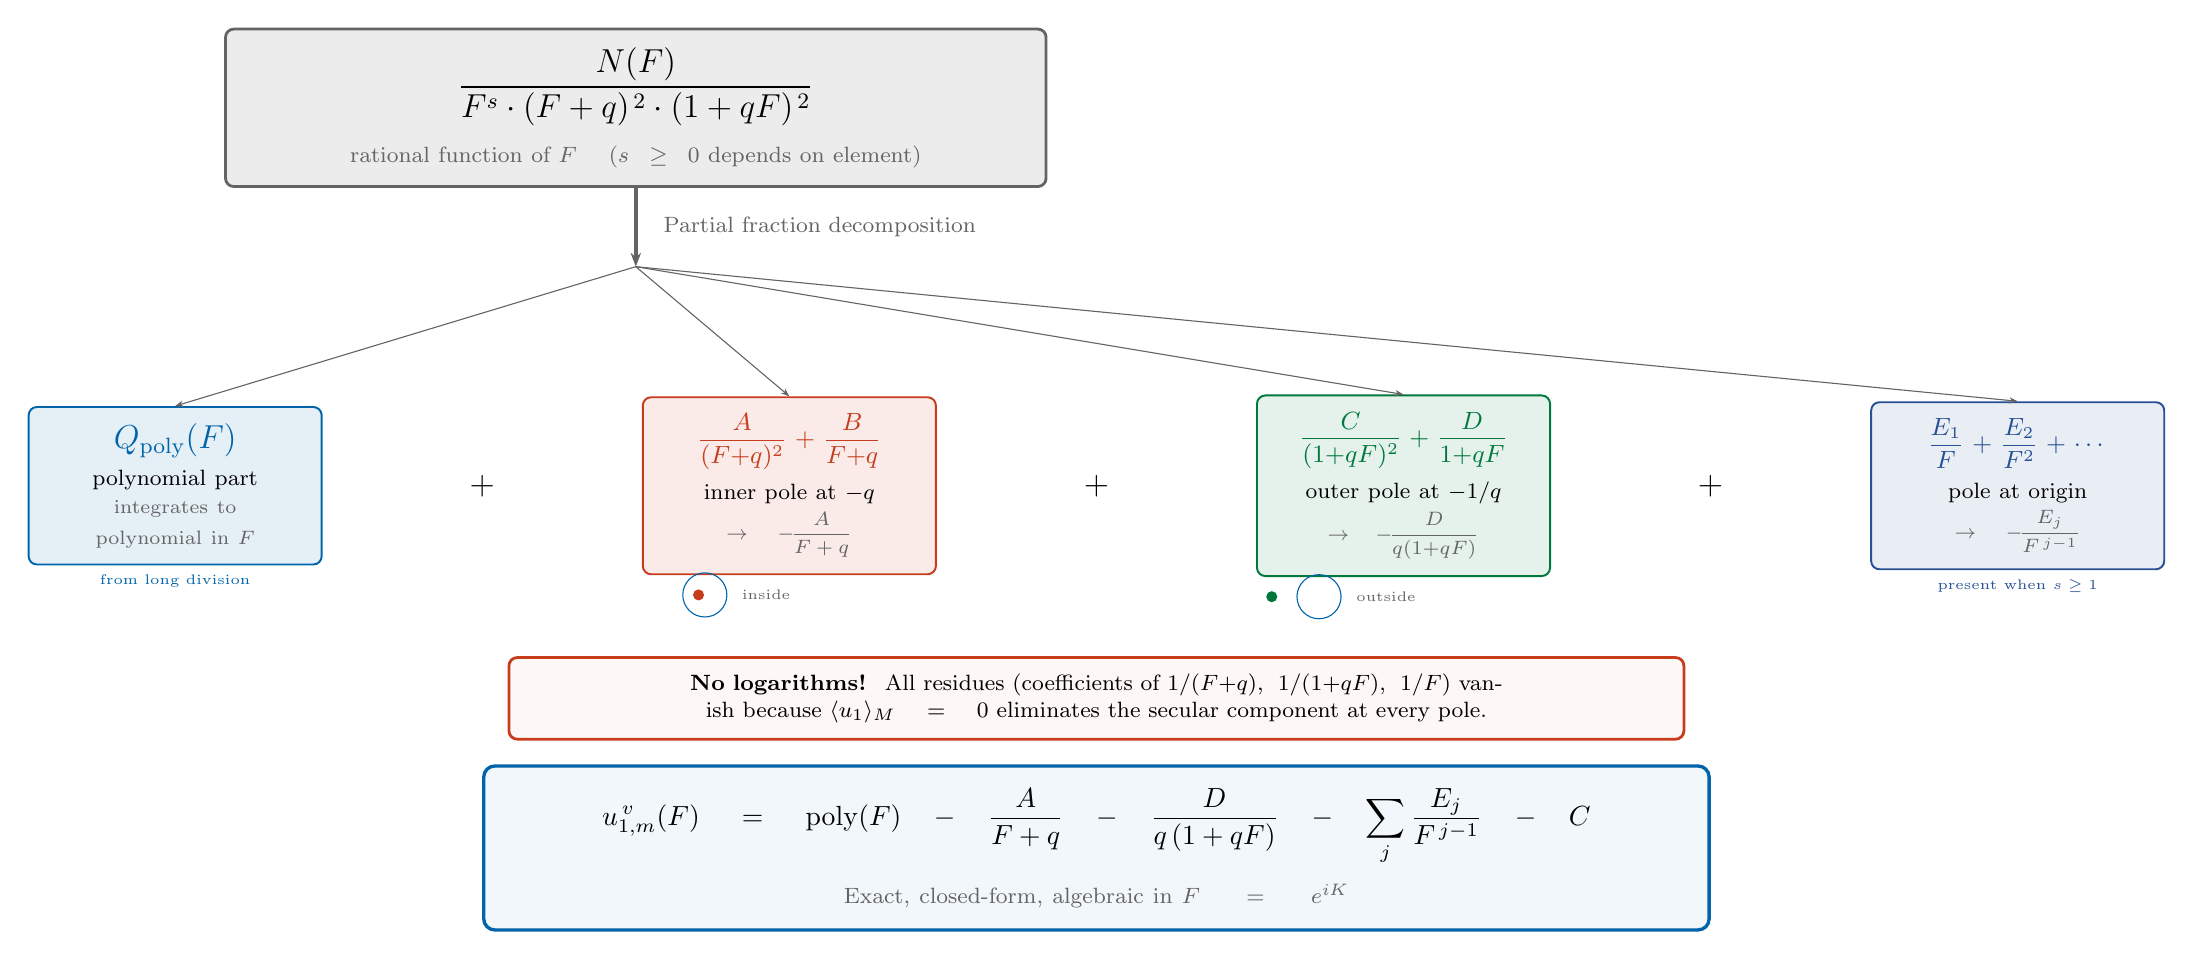
\begin{tikzpicture}[>=latex, font=\small,
  box/.style={draw, rounded corners=3pt, inner sep=6pt, minimum height=2.0cm,
              text width=3.3cm, align=center, line width=0.7pt},
  ]

% Center of the layout
\def\cx{5.85}

% ======================================================================
% TOP: Full integrand box
% ======================================================================
\node[box, fill=orbitgray!12, draw=orbitgray, text width=10cm,
      minimum height=2.0cm, line width=1pt]
  (integrand) at (\cx, 0)
  {%
    \large
    $\displaystyle \frac{N(F)}%
      {F^s \cdot (F+q)^{\,2} \cdot (1+qF)^{\,2}}$
    \\[6pt]
    \footnotesize\color{orbitgray}
    rational function of $F$ \quad
    ($s \ge 0$ depends on element)
  };

% ======================================================================
% Decomposition arrow
% ======================================================================
\draw[-{Stealth[length=5pt]}, line width=1.5pt, orbitgray]
  (integrand.south) -- ++(0, -1.0)
  node[midway, right=6pt, font=\footnotesize, orbitgray]
    {Partial fraction decomposition};

% ======================================================================
% BOTTOM ROW: Four component boxes, centered
% ======================================================================
\def\boty{-4.8}
\def\boxsep{3.9}

% Box positions: cx - 1.5*sep, cx - 0.5*sep, cx + 0.5*sep, cx + 1.5*sep
% so they center on cx

% --- Box A: polynomial part ---
\node[box, fill=accent!10, draw=accent]
  (boxA) at ({\cx-1.5*\boxsep}, \boty)
  {%
    \color{accent}\large $Q_{\mathrm{poly}}(F)$
    \\[4pt]
    \footnotesize\color{black}
    polynomial part
    \\[2pt]
    \scriptsize\color{orbitgray}
    integrates to\\polynomial in $F$
  };
\node[font=\tiny, accent, anchor=north] at (boxA.south) {from long division};

% Plus sign
\node[font=\large] at ({\cx-0.5*\boxsep}, \boty) {$+$};

% --- Box B: inner pole ---
\node[box, fill=highlight!10, draw=highlight]
  (boxB) at ({\cx+0.5*\boxsep}, \boty)
  {%
    \color{highlight}
    $\displaystyle \frac{A}{(F{+}q)^2} + \frac{B}{F{+}q}$
    \\[4pt]
    \footnotesize\color{black}
    inner pole at $-q$
    \\[2pt]
    \scriptsize\color{orbitgray}
    $\to\; -\!\dfrac{A}{F+q}$
  };
% Small circle icon: pole inside unit circle
\begin{scope}[shift={([xshift=0.8cm, yshift=-0.25cm]boxB.south west)}]
  \draw[accent, thin] (0,0) circle (0.28);
  \fill[highlight] (-0.08, 0) circle (2pt);
  \node[font=\tiny, orbitgray, anchor=west] at (0.35, 0) {inside};
\end{scope}

% Plus sign
\node[font=\large] at ({\cx+1.5*\boxsep}, \boty) {$+$};

% --- Box C: outer pole ---
\node[box, fill=darkgreen!10, draw=darkgreen]
  (boxC) at ({\cx+2.5*\boxsep}, \boty)
  {%
    \color{darkgreen}
    $\displaystyle \frac{C}{(1{+}qF)^2} + \frac{D}{1{+}qF}$
    \\[4pt]
    \footnotesize\color{black}
    outer pole at $-1/q$
    \\[2pt]
    \scriptsize\color{orbitgray}
    $\to\; -\!\dfrac{D}{q(1{+}qF)}$
  };
% Small circle icon: pole outside unit circle
\begin{scope}[shift={([xshift=0.8cm, yshift=-0.25cm]boxC.south west)}]
  \draw[accent, thin] (0,0) circle (0.28);
  \fill[darkgreen] (-0.6, 0) circle (2pt);
  \node[font=\tiny, orbitgray, anchor=west] at (0.35, 0) {outside};
\end{scope}

% Plus sign
\node[font=\large] at ({\cx+3.5*\boxsep}, \boty) {$+$};

% --- Box D: origin pole ---
\node[box, fill=earthblue!10, draw=earthblue]
  (boxD) at ({\cx+4.5*\boxsep}, \boty)
  {%
    \color{earthblue}
    $\displaystyle \frac{E_1}{F} + \frac{E_2}{F^2} + \cdots$
    \\[4pt]
    \footnotesize\color{black}
    pole at origin
    \\[2pt]
    \scriptsize\color{orbitgray}
    $\to\; -\!\dfrac{E_j}{F^{\,j-1}}$
  };
\node[font=\tiny, earthblue, anchor=north] at (boxD.south)
  {present when $s \ge 1$};

% ======================================================================
% Arrows from integrand to each box
% ======================================================================
\coordinate (fan) at ([yshift=-1.0cm]integrand.south);
\foreach \b in {boxA, boxB, boxC, boxD} {
  \draw[orbitgray, thin, -{Stealth[length=3pt]}]
    (fan) -- (\b.north);
}

% ======================================================================
% Key structural guarantee (annotation box)
% ======================================================================
\node[draw=highlight, rounded corners=3pt, line width=1pt,
      inner sep=6pt, text width=14.5cm, align=center,
      fill=highlight!4, font=\footnotesize]
  (nolog) at ({\cx+1.5*\boxsep}, \boty - 2.7)
  {%
    \textbf{No logarithms!}\;
    All residues (coefficients of $1/(F{+}q)$,\; $1/(1{+}qF)$,\; $1/F$)
    vanish because $\langle u_1 \rangle_M = 0$ eliminates the
    secular component at every pole.
  };

% ======================================================================
% Result box at very bottom
% ======================================================================
\node[draw=accent, rounded corners=4pt, line width=1.2pt,
      inner sep=8pt, text width=15cm, align=center,
      fill=accent!5, font=\normalsize]
  (result) at ({\cx+1.5*\boxsep}, \boty - 4.6)
  {%
    $\displaystyle
      u_{1,m}^{\,v}(F)
      \;=\; \mathrm{poly}(F)
      \;-\; \frac{A}{F+q}
      \;-\; \frac{D}{q\,(1+qF)}
      \;-\; \sum_{j} \frac{E_j}{F^{\,j-1}}
      \;-\; C$
    \\[6pt]
    \footnotesize\color{orbitgray}
    Exact, closed-form, algebraic in $F = e^{iK}$
  };

\end{tikzpicture}
\end{document}
